%% Template para dissertacao/tese na classe UFBAthesis
%% versao 1.0
%% (c) 2005 Paulo G. S. Fonseca
%% (c) 2012 Antonio Terceiro
%% (c) 2014 Christina von Flach
%% www.dcc.ufba.br/~flach/ufbathesis

%% Carrega a classe ufbathesis
%% Opcoes: * Idiomas
%%           pt   - portugues (padrao)
%%           en   - ingles
%%         * Tipo do Texto
%%           bsc  - para monografias de graduacao
%%           msc  - para dissertacoes de mestrado (padrao)
%%           qual - exame de qualificacao de mestrado
%%           prop - exame de qualificacao de doutorado
%%           phd  - para teses de doutorado
%%         * Media
%%           scr  - para versao eletronica (PDF) / consulte o guia do usuario
%%         * Estilo
%%           classic - estilo original a la TAOCP (deprecated) - apesar de deprecated, manter esse.
%%           std     - novo estilo a la CUP (padrao)
%%         * Paginacao
%%           oneside - para impressao em face unica
%%           twoside - para impressao em frente e verso (padrao)

% Atenção: Manter 'classic' na declaracao abaixo:
\documentclass[bsc, classic, a4paper, oneside]{ufbathesis}

%% Preambulo:
\usepackage[utf8]{inputenc}
\usepackage{graphicx}
\usepackage{lipsum}
\usepackage{hyphenat}
\usepackage[usenames, dvipsnames, table]{xcolor}
\usepackage{booktabs}
\usepackage{pifont}
\usepackage{multirow}
\usepackage{listings}
\usepackage{colortbl}
\usepackage{xfrac}
\usepackage{float}
\usepackage[FIGTOPCAP]{subfigure}


% Universidade
\university{Universidade Federal da Bahia}

% Endereco (cidade)
\address{Salvador}

% Instituto ou Centro Academico
\institute{Instituto de Matemática}

% Nome da biblioteca - usado na ficha catalografica
\library{Biblioteca Reitor Macêdo Costa}

% Programa de pos-graduacao
\program{Departamento de Ciência da Computação}

% Area de titulacao
\majorfield{Sistemas de Informação}

% Titulo da dissertacao
\title{Um método sensível ao contexto para predição de momentos oportunos para interrupção de motoristas}

% Data da defesa
% e.g. \date{19 de fevereiro de 2013}
\date{06 de agosto de 2017}
% e.g. \defenseyear{2013}
\defenseyear{2017}

% Autor
% e.g. \author{Jose da Silva}
\author{José Lucas dos Santos Borges}

% Orientador(a)
% Opcao: [f] - para orientador do sexo feminino
% e.g. \adviser[f]{Profa. Dra. Maria Santos}
\adviser[f]{Vaninha Vieira dos Santos}

% Orientador(a)
% Opcao: [f] - para orientador do sexo feminino
% e.g. \coadviser{Prof. Dr. Pedro Pedreira}
% Comente se nao ha co-orientador
% \coadviser{Rogerio de Carvalho Bastos}
% \coadviser{Ítalo Valcy da Silva Brito}
\coadviser{Alberto Vianna Dias da Silva}

%% Inicio do documento
\begin{document}

\pgcompfrontpage

%% Parte pre-textual
\frontmatter

\pgcomppresentationpage

%%%%%%%%%%%%%%%%%%%%%%%%%
% Ficha catalografica
%%%%%%%%%%%%%%%%%%%%%%%%%

\authorcitationname{Borges, José Lucas dos Santos} % e.g. Terceiro, Antonio Soares de Azevedo
\advisercitationname{dos Santos, Vaninha Vieira} % e.g. Chavez, Christina von Flach Garcia
\catalogtype{Monografia (Graduação)} % e.g. ou ``Tese (Doutorado)''

\catalogtopics{1. Contexto.}
% Listar palavras-chave do trabalho para a FICHA CATALOGRAFICA}, por exemplo,
% ``1. Complexidade Estrutural. 2. Qualidade de Software 3. Engenharia de Software''
\catalogcdd{XXX.XX} % e.g.  XXX.XX (número nesse formato serah dado pela biblioteca)
\catalogcdu{XXX.XX.XXX} % e.g.  XXX.XX.XXX (idem)
\catalogingsheet

%%%%%%%%%%%%%%%%%%%%%
% Termo de aprovacaoo
%%%%%%%%%%%%%%%%%%%%%

\approvalsheet{Salvador, DIA de MES de ANO}{
   \comittemember{Profa. Dra. Vaninha Vieira dos Santos}{Universidade Federal da Bahia}
   \comittemember{Ítalo Valcy da Silva Brito}{Universidade Federal da Bahia}
   % Para mestrado, apenas 3.
   % \comittemember{Prof. Dr. Professor 4}{Universidade HJKL}
   % \comittemember{Profa. Dra. Professora 5}{Universidade QWERTY}
}

%%%%%%%%%%%%%%%%%%%%%%%%%%%%%%%%%%%%%%%%
% Dedicatoria, Agradecimentos, Epigrafe
%%%%%%%%%%%%%%%%%%%%%%%%%%%%%%%%%%%%%%%%

% Comente para ocultar
\begin{dedicatory}
DIGITE A DEDICATORIA AQUI
\end{dedicatory}

% Agradecimentos
% Se preferir, crie um arquivo `a parte e o inclua via \include{}
\acknowledgements
DIGITE OS AGRADECIMENTOS AQUI

% Epigrafe
\begin{epigraph}[NOTA]{AUTOR}
DIGITE AQUI A CITACAO
\end{epigraph}

%%%%%%%%%%%%%%%%%%%%%
% Resumo em Portugues
%%%%%%%%%%%%%%%%%%%%%

\resumo
A notificação inoportuna de motoristas é um problema real que pode causar distrações e interrupções no trânsito e
consequentemente acidentes. Em geral, as pessoas levam até 27\% mais tempo para concluir uma tarefa quando são interrompidas
e tendem a cometer o dobro de erros. Um dos meios pelos quais motoristas recebem interrupções são via notificações
em dispositivos móveis, que podem chegar à ordem de centenas por dia. Apesar disso, mesmo sabendo de sua capacidade
interruptiva, notificações são valorizadas pelos usuários e fazem parte do próprio hábito de uso dos smartphones.
Sendo assim, como diminuir o potencial interruptivo das notificações para os motoristas sem eliminá-las completamente?

Para tentar mitigar este problema, o presente trabalho propõe a construção de um sistema de notificação sensível ao
contexto com identificação de momentos oportunos e inoportunos para notificação de motoristas. O sistema proposto usa
apenas sensores de smartphone (giroscópio e GPS) para alcançar este objetivo, e infere se o motorista pode ser
interrompido em um dado momento. Um experimento de avaliação foi conduzido com motoristas em situações reais de direção
para verificar se o sistema conseguia identificar momentos oportunos e inoportunos para notificar apropriadamente. Ao
final do experimento apurou-se que o sistema obteve uma acurácia de 88\%.

\begin{keywords}
Interrupção, notificação, motoristas, contexto.
\end{keywords}


%%%%%%%%%%%%%%%%%%%
% Resumo em Ingles
%%%%%%%%%%%%%%%%%%%

\abstract
Inopportune driver notifications is a real problem that may cause distractions and interruptions in traffic and
hence accidents. People usually take 27\% more time to finish a task when they are interrupted and tend to commit the
double amount of mistakes. One of the ways by which drivers are interrupted it's with notifications on mobile devices,
that may reach extremely high amounts in a normal day. Despite that, notifications are valued by users and they are
part of the common use of smartphones. Therefore, how to lessen the interruptive potential of notifications without
eliminating them completely?

To mitigate this problem, the present work propose the development of a context-aware notification system with opportune
and inopportune moments identification for drivers notification. The proposed system use only smartphone sensors (gyroscope
and GPS) to achieve this objective, and infer if the driver may be interrupted in the moment. Experiments were performed with
people in real driving situations to verify if the system could identify opportune and inopportune moments to notify properly.
At the end of the experiments the system obtained an accuracy of 88\%.

\begin{keywords}
Interruption, notification, drivers, context.
\end{keywords}



%%%%%%%%%%%%%%%%%%%
% Sumario / Indice
%%%%%%%%%%%%%%%%%%%

% Comente para ocultar
\tableofcontents

% Lista de figuras
% Comente para ocultar
\listoffigures

% Lista de tabelas
% Comente para ocultar
\listoftables

%% Parte textual
\mainmatter

% Eh aconselhavel criar cada capitulo em um arquivo separado, digamos
% "capitulo1.tex", "capitulo2.tex", ... "capituloN.tex" e depois
% inclui-los com:
% \include{capitulo1}
% \include{capitulo2}
% ...
% \include{capituloN}
%
% Importante:
% Use \xchapter{}{} ao inves de \chapter{}; se não quiser colocar texto antes do inicio do capitulo, use \xchapter{texto}{}.

\xchapter{Introdução}{}
\label{introducao}

Dirigir um veículo pode ser considerado uma tarefa complexa, já que envolve diversas pequenas ações coordenadas
que dependem tanto de fatores externos quanto internos. Um motorista deve saber adaptar-se a diferentes situações,
agir apropriadamente perante cada uma delas e tomar medidas rápidas em caso de emergência.

Neste contexto, a interrupção inoportuna é um perigo que pode ser fatal, pois demanda atenção do motorista em um momento
onde a distração pode levar a um acidente. Um fato que corrobora isto é o de que pessoas levam até 27\% mais tempo para
concluir uma tarefa quando são interrompidas e tendem a cometer o dobro de erros \cite{bailey2006need}. Exemplos de
interrupções que podem ocorrer para motoristas são barulhos repentinos, conversas com passageiros e notificações em
seu celular.

Outra informação que sustenta esta hipótese é a de que ao demandar a atenção dos motoristas durante a execução de
tarefas complexas sua distração também aumenta, pois a quantidade de informação que um motorista pode assimilar
depende da complexidade de sua tarefa no momento \cite{schneegass2013data}.

Um dos meios pelos quais os motoristas recebem interrupções são via notificações em dispositivos móveis.
Diariamente, pessoas que utilizam qualquer tipo de dispositivo móvel recebem dezenas de notificações
\cite{pielot2014situ}. Tais notificações demandam a atenção do usuário e podem acabar interrompendo uma tarefa que
está sendo executada no momento, dado que a atenção humana é um recurso finito \cite{simon1971designing}.

Interrupções de motoristas já são um problema a ser considerado. Nos Estados Unidos, 10\% dos acidentes com morte, em 2014, tiveram relação
com algum tipo de distração e 13\% deste tipo de distrações estão relacionadas com o uso de celulares e \textit{smartphones}
\cite{distracted2014}. Diante disto, prevenir este tipo de distração relacionada a dispositivos móveis torna-se uma necessidade.

A utilização de dispositivos móveis durante a direção de veículos, apesar de ser proibido no Brasil, é liberado em alguns
outros países, como Estados Unidos (em alguns estados como Flórida e Colorado \cite{cellphoneuse, distracteddriving} e Suécia \cite{swedendrive}.

Ao identificar padrões nos dados contextuais que indiquem momentos oportunos para interromper motoristas, é possível
construir uma solução que os notifique apropriadamente a depender do contexto que eles se encontram. Este trabalho propõe
o desenvolvimento de um sistema sensível ao contexto que detecte momentos oportunos e inoportunos para notificação de motoristas, utilizando
apenas sensores de smartphone. Este módulo será incorporado ao aplicativo Meu Possante, que serve como um auxiliar de mecânica automotiva.

O módulo supracitado será responsável por gerenciar o momento de entrega das notificações geradas pelo Meu Possante ao dispositivo. Ao
incluí-lo no código há uma melhoria na segurança do usuário, já que as notificações não serão entregues em momentos indevidos e
colocando em risco a vida dos mesmos quando estiverem dirigindo.

Neste trabalho a seguinte metodologia foi utilizada: inicialmente investigamos momentos oportunos e inoportunos para interrupção de motoristas
a partir da leitura de artigos da área. Tendo em mente os momentos escolhidos para este trabalho (curvas, mudança de faixa, veículo parado e
velocidade baixa e constante), buscamos limiares na literatura que nos permitam identificá-los utilizando apenas sensores de smartphone.
Com estes dados em mãos, um módulo foi desenvolvido em Android nativo e incorporado em um aplicativo experimental. Por fim, elaboramos um
experimento para avaliar a solução proposta.

O experimento foi feito com três motoristas em situações reais de direção, e um total de xxxx amostras foram coletadas. Os resultados mostraram
lorem ipsum.

Os próximos capítulos estão estruturados da seguinte forma: O Capítulo \ref{meupossante} apresenta uma visão geral sobre o aplicativo Meu Possante,
motivador deste trabalho. O Capítulo \ref{revisao-lit} discorre sobre os conceitos teóricos importantes para o entendimento deste trabalho e
apresenta os trabalhos relacionados. O Capítulo \ref{proposta} apresenta a proposta deste trabalho, um sistema sensível ao contexto que detecta
momentos oportunos e inoportunos para notificação de motoristas. O Capítulo \ref{estudo-experimental} apresenta o experimento de avaliação realizado e
os resultados obtidos. Por fim, no Capítulo \ref{conclusao} são apresentadas as considerações finais.

\xchapter{Meu Possante}{}
\label{meupossante}
Mecânica automotiva é um assunto extremamente complexo. Cada um dos inúmeros componentes
do automóvel tem seu próprio ciclo de vida e devem ser revisados e trocados em seu próprio
tempo. Além disso, certas condições de uso podem diminuir a vida útil de algumas peças,
tornando mais frequente a necessidade de revisão.

A falta de conhecimento destes fatos pode levar ao dono de um automóvel negligenciar
as manutenções no tempo correto, causando desde transtornos que poderiam ser facilmente
evitados a acidentes ocasionados por falhas mecânicas.

Em 2016, mais de 2 milhões de automóveis foram vendidos no Brasil
\cite{fenabrave}. Dentre este número, é seguro assumir que poucos de seus
proprietários são especialistas em mecânica e possuem dúvidas sobre o
funcionamento das peças do seu veículo, além de não saber exatamente em qual
momento deve-se trocar cada uma de suas peças. Estas informações geralmente
estão no manual do veículo, mas é inviável para uma pessoa leiga memorizar
todas estas informações.

Após a compra de um automóvel, a sua manutenção é de inteira responsabilidade
do proprietário. Todas as operações de manutenção, especificadas pelo fabricante,
devem ser realizadas dentro dos intervalos apropriados \cite{manualhyundai}.
Proporcionar manutenção apropriada para o veículo, não somente reduz os custos
operacionais, mas também ajuda a impedir mau funcionamento devido a negligência,
caso que geralmente não é coberto por garantia \cite{manualonix}.

Para executar a manutenção apropriadamente, o proprietário precisa estar
sempre atento ao momento correto da troca das peças, que muda de acordo
com as condições de uso de um carro. Acompanhar estas diferentes variáveis pode
ser difícil para pessoas comuns.

O uso de um aplicativo para celular pode ser uma grande ajuda na decisão de quando
é necessário a revisão e troca de peças, alertando o usuário visualmente quando alguma
manutenção está próxima. Neste sentido surge o Meu Possante, um aplicativo que monitora
o estado atual do veículo e avisa o momento em que as manutenções das peças serão
necessárias.

\section{O aplicativo em linhas gerais (provisório)}
\label{meupossante-app}

O Meu Possante possui um objetivo simples: Auxiliar o motorista a identificar quais
peças de seu carro precisarão de manutenção em um futuro próximo. O aplicativo nasceu
como trabalho final da disciplina de Desenvolvimento de Aplicações para Dispositivos
Móveis e está em processo refinamento para publicação na Google Play Store.

A tela principal do aplicativo mostra todos os componentes do veículo que são monitorados,
como pode ser visto na figura \ref{meu-possante-tela-principal}. Ao clicar em um componente,
a tela do mesmo é mostrada, com informações como a frequência de troca e quilometragem
atual.

\begin{figure}[h]
\centering
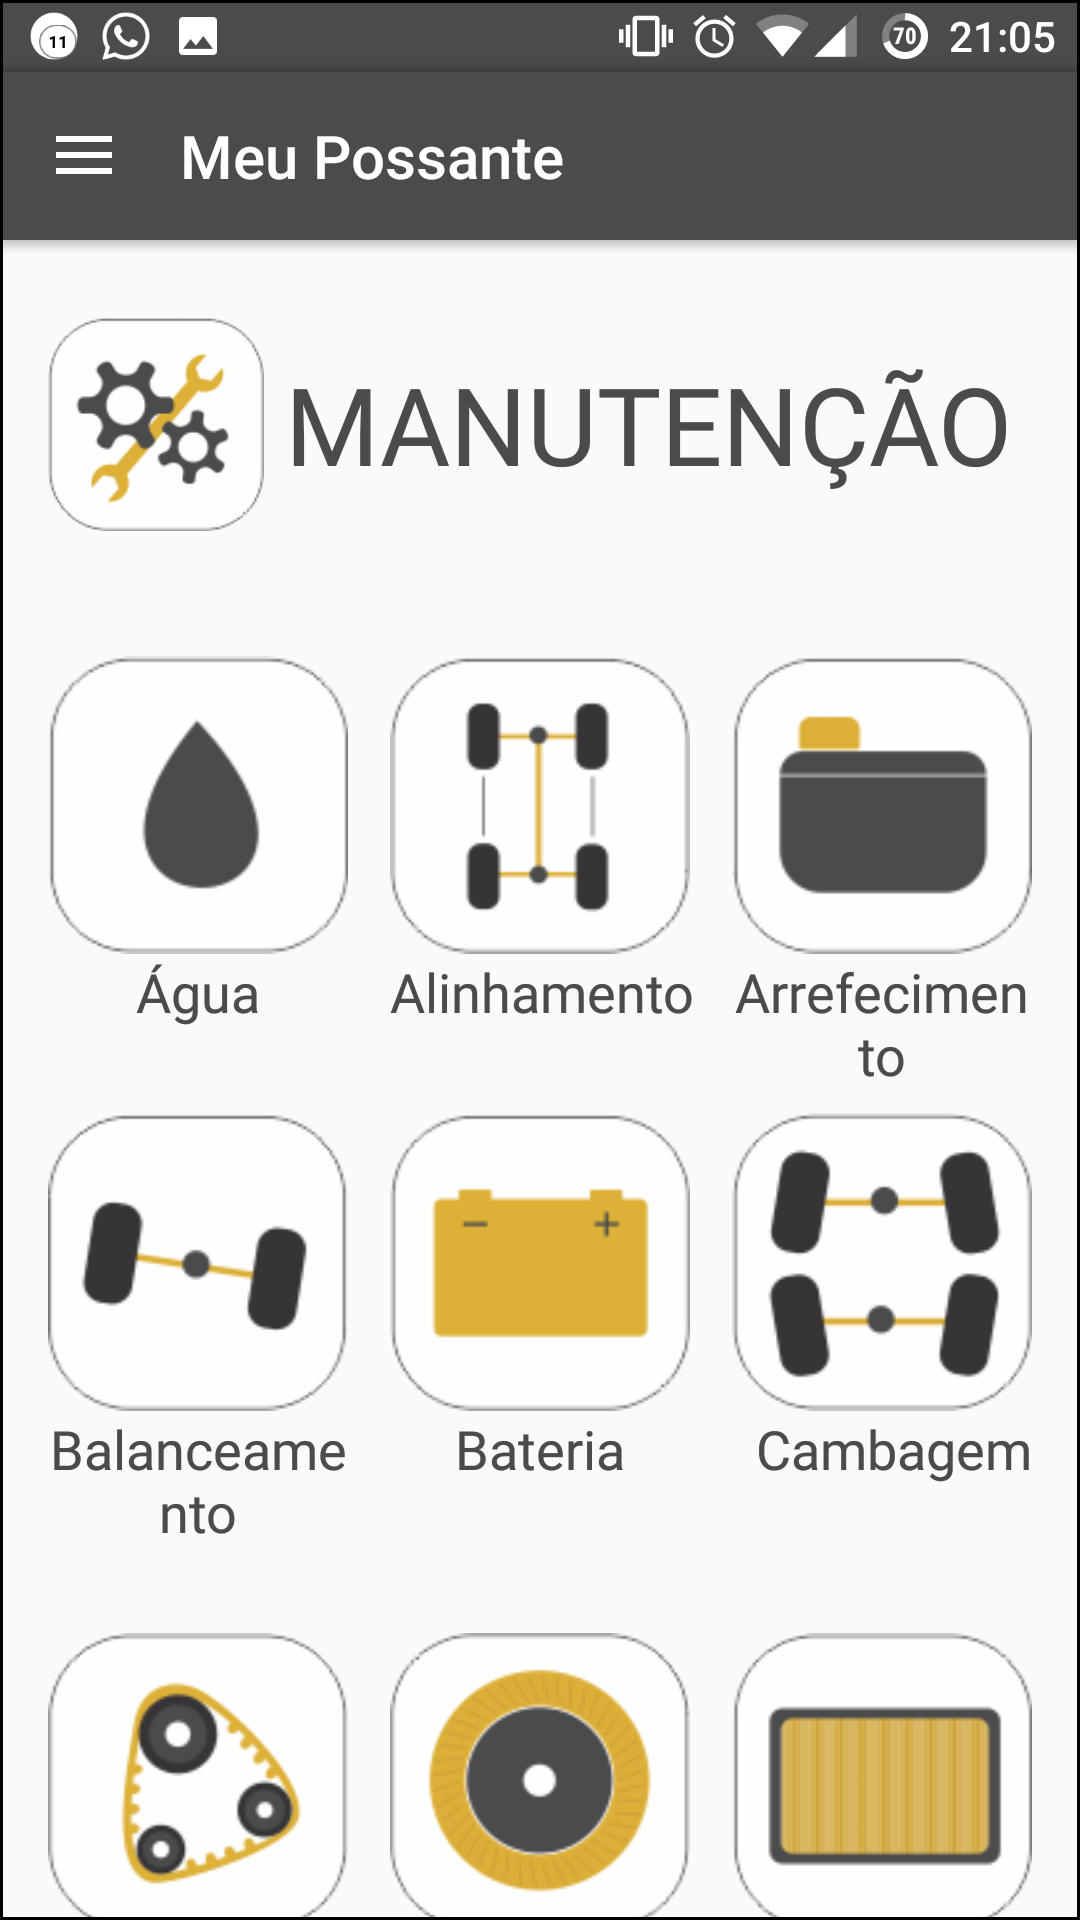
\includegraphics[width=0.3\textwidth]{images/meu-possante-tela-principal.png}
\caption{Tela principal do Meu Possante}
\label{meu-possante-tela-principal}
\end{figure}

O aplicativo utiliza informações do GPS do dispositivo para calcular a distância percorrida
pelo motorista enquanto está dirigindo. No momento em que detecta a iminência de manutenção
de alguma das peças do veículo, uma notificação é enviada para o dispositivo do usuário.
Esta notificação leva à página da peça correspondente no aplicativo, onde pode ser lido
mais detalhes sobre o estado atual, como a quilometragem e qual a quilometragem da
próxima troca, como pode ser visto na figura \ref{meu-possante-tela-componente}.

\begin{figure}[h]
\centering
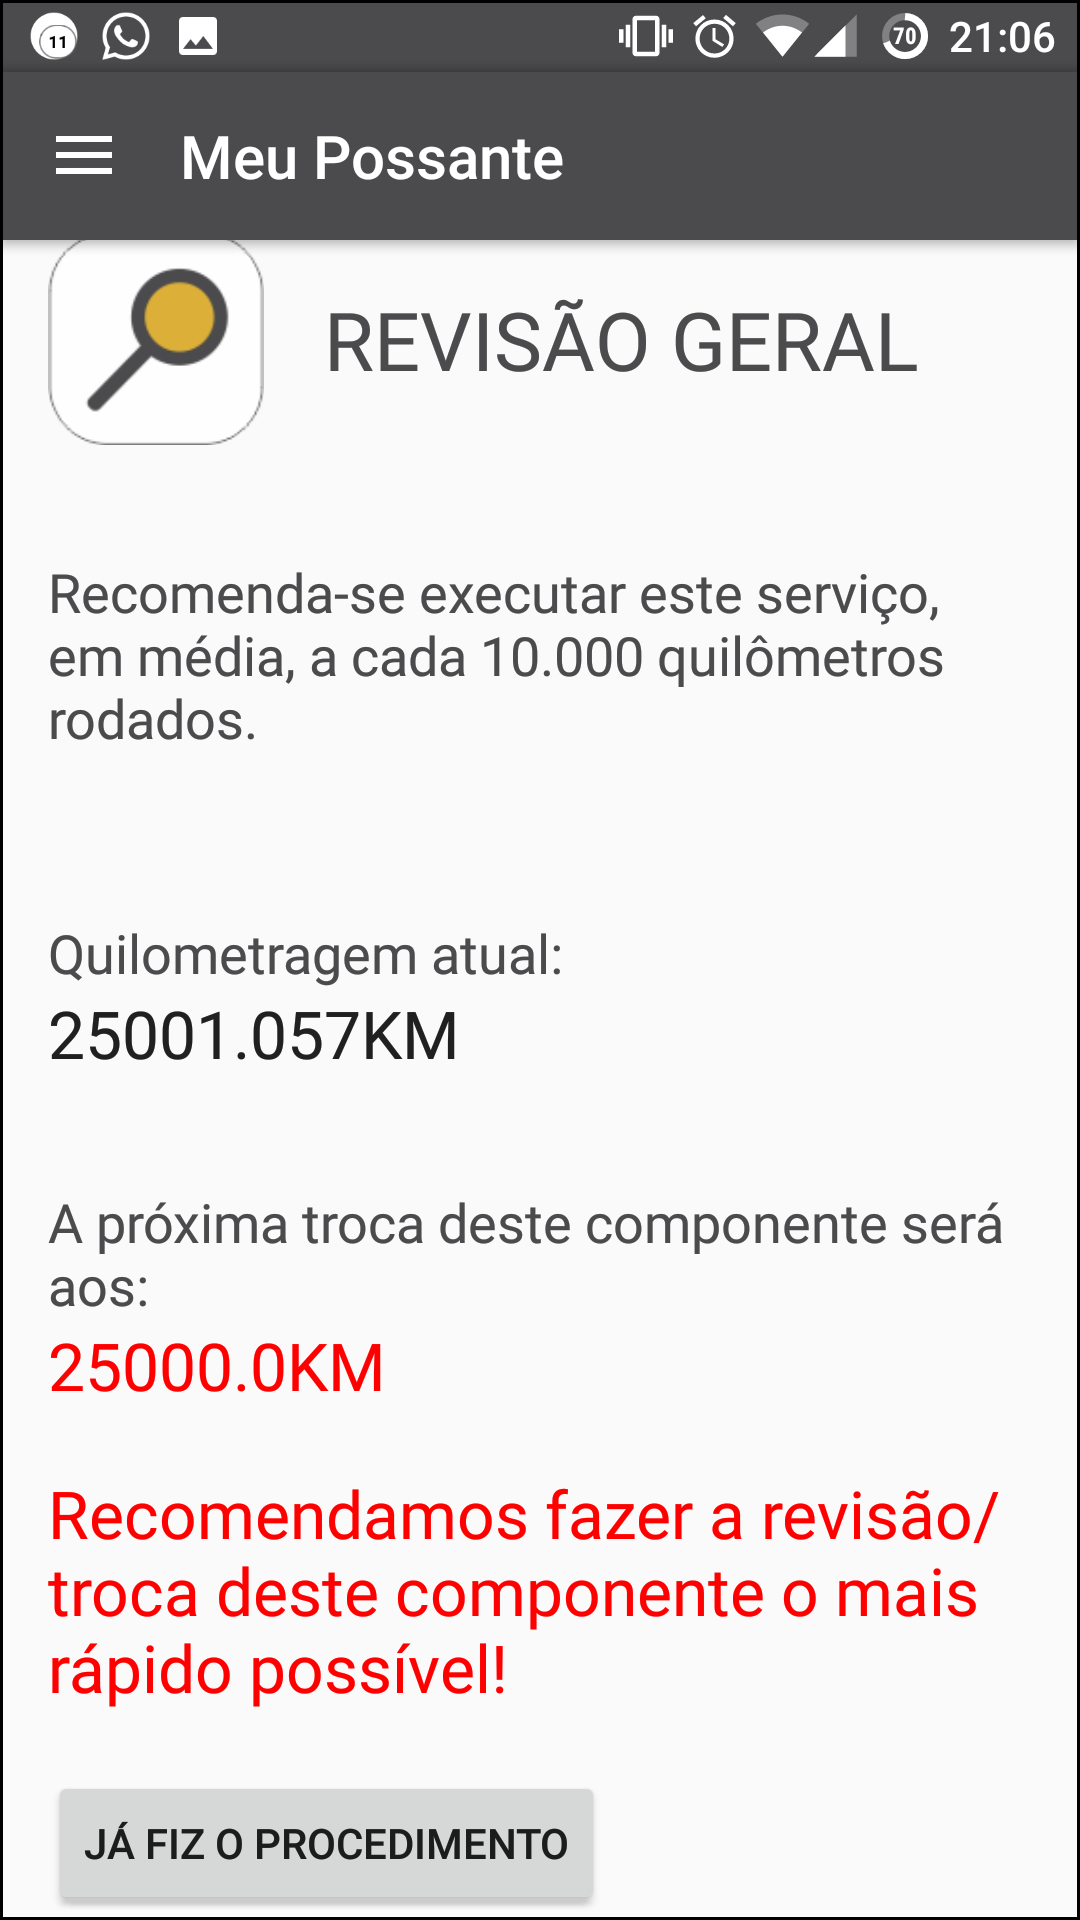
\includegraphics[width=0.3\textwidth]{images/meu-possante-tela-componente.png}
\caption{Tela que indica a necessidade de revisão de um componente}
\label{meu-possante-tela-componente}
\end{figure}

Na versão atual, o motorista precisa indicar que está dirigindo através de uma tela
específica. Ao indicar que está dirigindo, o aplicativo começa a monitorar a localização
do usuário e seu deslocamento

\xchapter{Revisão da Literatura}{}
\label{revisao-lit}
Este capítulo aborda os principais fundamentos teóricos envolvidos na notificação oportuna de motoristas,
tema central deste trabalho, e traz uma revisão dos trabalhos relacionados com o tema. As seções deste capítulo
estão estruturadas da seguinte forma: A seção \ref{interrupcao} apresenta os principais conceitos sobre interrupção
e seus efeitos sobre os motoristas. A seção \ref{notificacao} fala sobre as notificações e seu efeito interruptivo.
A seção \ref{contexto} discorre sobre contexto. Por fim, a seção \ref{trabalhos-relacionados} apresenta os trabalhos
correlatos com o presente trabalho.

\section{Interrupção}
\label{interrupcao}
Controle cognitivo é o processo que permite que o comportamento do indíviduo e seu processamento de informação variem de momento a
momento, ao invés de se manterem rígidos e inflexíveis. O controle cognitivo pode ser expresso de várias maneiras, uma das quais
envolve a seleção do próximo pensamento para se focar, quando há múltiplas opções e quando distrações podem intervir.

Um exemplo do fato acima é uma conversação, que geralmente segue uma linha coerente. Se uma interrupção ocorre (um dos celulares dos
interlocutores começa a tocar, por exemplo) esta linha pode ser perdida, levando-os a se perguntar "Onde nós estávamos?" \cite{altmann2014momentary}.

Segundo \citeonline{ferreira2004novo}, interrupção é aquilo que faz parar uma ação ou um estado; o ato de cortar a continuidade de
algo. \citeonline{mcfarlane1997interruption} define interrupção humana como o processo de coordenar mudanças abruptas em uma atividade.

A interrupção durante a execução de uma tarefa pode ter vários efeitos adversos. \citeonline{lewin1927untersuchungen} diz
que pessoas lembram melhor dos detalhes de tarefas que não foram interrompidas. \citeonline{zijlstra1999temporal} concluem que
pessoas cometem mais erros em tarefas após uma interrupção. \citeonline{gillie1989makes} afirmam que as pessoas executam tarefas
mais vagarosamente após uma interrupção, se comparado com a performance pré-interrupção. Diante destas evidências, pode-se
afirmar que interrupções durante uma tarefa são bastante nocivas para a execução da mesma.

\subsection{Interrupção de Motoristas}
\label{interrupcao-motoristas}

Trabalhos anteriores estudaram os efeitos da execução de tarefas concorrentes com a direção. \citeonline{monk2004recovering} citam
que há diversos efeitos adversos ao executar tarefas cognitivas complexas durante a direção, como atraso na resposta a
acontecimentos repentinos, desatenção a informações sinalizadas, diminuição do controle do veículo, estreitamento do campo
de visão e mudanças de comportamento de frenagem e direção.

Além disso, vários problemas na execução de uma tarefa após uma interrupção, como os citados na seção \ref{interrupcao}, afetam o
motorista durante a direção de um veículo:

\begin{itemize}
  \item Ao não lembrar de detalhes do que estava fazendo antes da interrupção, o motorista pode esquecer de informações
  apontadas pela sinalização de trânsito;
  \item Ao cometer erros após uma interrupção, o motorista põe em risco a si mesmo e a seus pares, podendo causar acidentes
  de trânsito;
  \item Ao reagir mais vagarosamente após uma interrupção, o motorista fica vulnerável a ameaças externas que exijam de sua
  capacidade reativa;
\end{itemize}

O estudo de \citeonline{monk2004recovering} ainda conclui que interrupções antes ou depois de uma tarefa ou sub-tarefa trazem
menos problemas, e cita curvas, mudanças de faixa e entrada em uma rodovia como exemplos de sub-tarefas que o motorista executa.
Este fato serve de justificativa para a escolha dos momentos inoportunos a serem detectados neste trabalho, que são a curva
e mudança de faixa.

Estima-se que o uso de celular durante o ato de dirigir um veículo aumenta o risco de acidentes em 38\% \cite{laberge2001wireless}.
Em paralelo a este fato, \citeonline{stothart2015attentional} afirmam que apenas o ato de receber uma notificação, mesmo que ela não seja
atendida, distrai o motorista tanto quanto receber uma ligação no celular ou responder uma mensagem de texto. Ante este fato, é
necessário estudar as notificações e sua capacidade de interromper tarefas.

\section{Notificações e seu caráter interruptivo}
\label{notificacao}

Notificação pode ser definida como um sinal visual, audível ou táctil, gerado por uma aplicação
ou serviço e que passa informação para um usuário que está fora de seu foco de atenção \cite{iqbal2010notifications}.
Em dispositivos móveis, notificações geralmente são enviadas instantaneamente no momento em que ocorre alguma atividade que pode ser relevante
para o usuário quando a aplicação não está aberta, ex: um email novo, uma mensagem de texto que acaba de chegar ou um
novo comentário em suas redes sociais. Em alguns casos o usuário toma ações imediatas após a chegada da notificação,
enquanto em outros ela é simplesmente ignorada. Essas ações dependem da importância da notificação e do contexto do
usuário \cite{sahami2014large}.

Em dispositivos móveis uma notificação é uma mensagem que pode ser exibida ao usuário fora da interface normal de um aplicativo.
Quando o aplicativo emite uma notificação, ela primeiro aparece como um ícone na área de notificação. No sistema operacional móvel
Android \cite{android}, para ver os detalhes da notificação, o usuário abre a gaveta de notificação \cite{notificationDrawer}. A Figura
\ref{notification-drawer} mostra o layout da gaveta de notificações no Android. Cada retângulo branco preenchido com ícones
e texto representa uma notificação diferente. O horário de chegada aparece no canto direito de cada notificação.

Notificações semelhantes geralmente são agrupadas para que não sejam exibidas inúmeras notificações com conteúdo parecido.
Pode-se perceber na Figura \ref{notification-drawer} que a maioria das notificações possui um indicativo de informações agrupadas
ao invés de múltiplas notificações. Ex: O texto "\textit{3 new messages}" que aponta que existem 3 novas mensagens, ao invés de 3
notificações apontando 1 nova mensagem cada.

A maioria das notificações possui pelo menos uma ação atrelada a si. Uma ação permite que os usuários passem
diretamente da notificação para uma tela específica do aplicativo, onde podem visualizar um ou mais eventos ou realizar
outros trabalhos.

\begin{figure}[h]
\centering
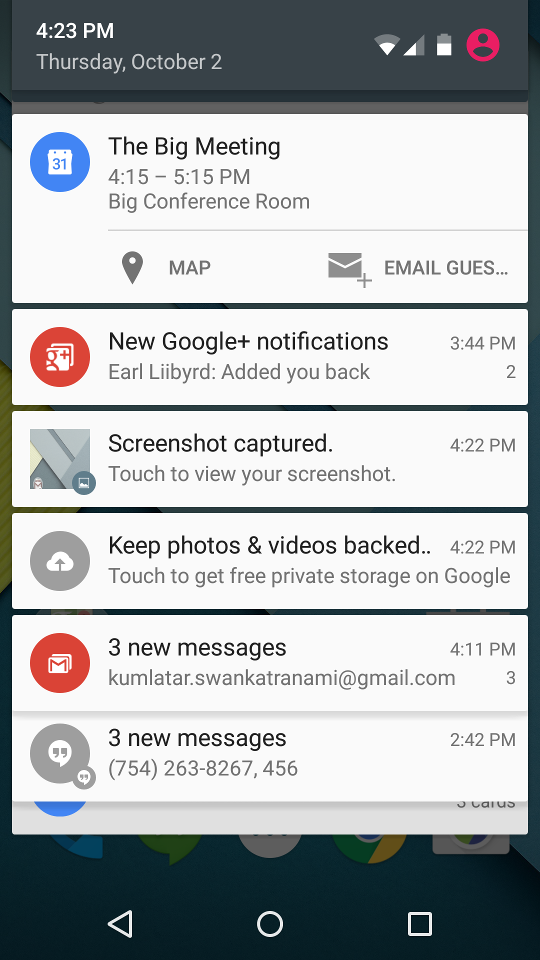
\includegraphics[width=0.3\textwidth]{images/notification_drawer.png}
\caption{Exemplo de notificações no Android \cite{notificationDrawer}}
\label{notification-drawer}
\end{figure}

A área de notificação e a gaveta de notificação mostradas na Figura \ref{notification-drawer} são áreas controladas pelo
sistema operacional e que o usuário pode visualizar a qualquer momento.

Cada vez que um dispositivo provê informação proativamente (ex: Notificando que há um novo comentário em suas redes
sociais) ele está competindo pela atenção do usuário e possívelmente interrompendo tarefas que estão acontecendo no momento
\cite{ho2005using}. Alguns estudos tentaram entender a relação dos usuários com este efeito adverso.

\citeonline{oulasvirta2012habits} discorrem sobre os hábitos de uso de smartphones. Os autores descobriram que o rápido acesso a
conteúdo dinâmico pode criar hábitos, que ficam mais fortes com o aumento da frequência de uso do dispositivo. Eles
também mencionam que estes hábitos são uma característica particular do uso de smartphones e que ainda não são percebidos
pela sociedade como problemáticos. \citeonline{iqbal2010notifications} concluem em seu estudo que usuários valorizam o sentimento
de informação que as notificações trazem e que, mesmo cientes de seus efeitos interruptivos, preferem manter este sentimento.

Estes achados permitem a conclusão que apesar de sua capacidade interruptiva, notificações são valorizadas pelos
usuários e fazem parte do próprio hábito de uso dos smartphones. Por este motivo, é necessário que se diminua o potencial
interruptivo das notificações, o que pode ser conseguido utilizando contexto, como sinalizam alguns autores
\cite{ho2005using, kern2003context, iqbal2010notifications}.

\section{Contexto}
\label{contexto}

Em 1991 é cunhado o termo "Computação Ubíqua", que se refere ao caráter invisível da integração de dispositivos
computacionais diversos e da adaptação dos mesmos à necessidade do usuário no momento \cite{weiser1991computer}.
Um elemento bastante importante para a Computação Ubíqua é o estudo do contexto.

Contexto é definido por \citeonline{dey2001understanding} como "Qualquer informação que pode ser utilizada para
caracterizar a situação de entidades (ex: um usuário, lugar ou objeto) e que é considerada relevante para
a interação entre um usuário e uma aplicação, incluindo o próprio usuário e aplicação". Esta definição é
a mais utilizada na área. Alguns exemplos de elementos de contexto são
localização do usuário, identidade do usuário e tempo \cite{ryan1999enhanced}.

Diversos sensores podem ser utilizados para determinar informações sobre o contexto do usuário. Alguns exemplos são
sensores de localização (GPS (\textit{Global Positioning System}, em português Sistema de Posicionamento Global)),
sensores de luz, acelerômetro e giroscópio.

Informações de contexto são importantes para definir o estado atual do usuário e do ambiente onde ele está inserido,
mas somente isto é insuficiente. Para utilizar estas informações satisfatoriamente é ideal que se construa um sistema
adaptativo e que supra as necessidades do usuário em tempo real utilizando as informações de contexto. Resumindo,
um sistema sensível ao contexto.

Sistemas sensíveis ao contexto são capazes de adaptar suas operações ao contexto atual, sem intervenção
explícita do usuário e têm como objetivo aumentar sua usabilidade e efetividade levando em conta elementos
de contexto \cite{baldauf2007survey}.  Um sistema é sensível ao contexto se ele utiliza contexto para prover
informações relevantes e/ou serviços para usuários, sendo que a relevância depende das tarefas do usuário
\cite{abowd1999towards}.

Este trabalho propõe a construção de uma ferramenta que utilize contexto para a detecção de momentos oportunos para
o envio de notificações a motoristas, utilizando apenas sensores de um smartphone comum.

\section{Trabalhos Relacionados}
\label{trabalhos-relacionados}

Em pesquisas preliminares não encontramos nenhuma aplicação, solução ou proposta que construiu um mecanismo para
notificação de motoristas em momentos oportunos utilizando contexto. Entretanto, encontramos projetos de aplicações que
usam dados de contexto para detectar aspectos relacionados ao comportamento de motoristas.

\citeonline{kim2015sensors} desenvolveram um classificador utilizando aprendizagem de máquina para detectar a interruptibilidade
de motoristas em um dado momento. Para a coleta de dados foram utilizados um sensor fisiológico vestível, quatro sensores
de movimento também vestíveis, câmeras direcionadas ao tráfego e ao motorista e um dispositivo OBD (\textit{On-Board Diagnostic},
em português Sistema de Diagnóstico de Bordo), como mostrado na figura \ref{kim-sensors}.

\begin{figure}[h]
\centering
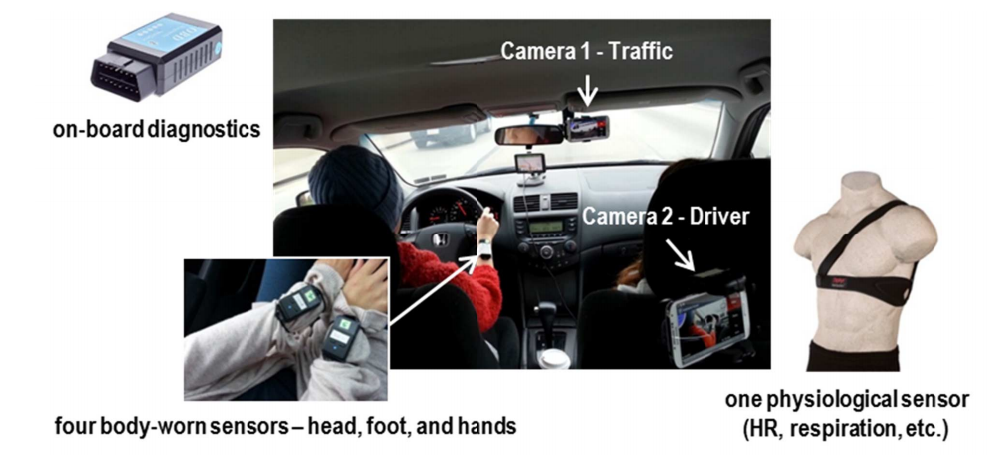
\includegraphics[width=0.9\textwidth]{images/kim-sensors.png}
\caption{Sensores utilizados no trabalho de \citeonline{kim2015sensors}.}
\label{kim-sensors}
\end{figure}

Um experimento foi feito com 25 motoristas (14 mulheres e 11 homens), com idade entre 19 e 69 anos, consistindo em 2 seções
onde os motoristas dirigiam de um ponto a outro. O resultado do experimento mostrou que interrupções têm menos impacto em um motorista
quando ele não está com nenhuma das mãos no volante ou quando está interagindo com um periférico (controlador do ar condicionado, por exemplo).
O classificador para detecção de interruptibilidade construído obteve 94\% de precisão na detecção de momentos
oportunos para interrupção de motoristas.

O trabalho de \citeonline{kim2015sensors} também apresenta evidências de que há outros momentos oportunos para interromper motoristas, como
por exemplo quando o carro está parado (todas as vezes em que o motorista não tinha nenhuma das mãos no volante, a velocidade do carro era menor
do que 3 km/h), quando a velocidade do carro é baixa e quando a velocidade é constante. Estes achados servem como justificativa para a
escolha dos momentos oportunos a serem detectados neste trabalho, que são o veículo parado e a velocidade baixa e constante.

%O presente trabalho visa construir um classificador semelhante, com o diferencial de utilizar apenas sensores de smartphone.

\citeonline{johnson2011driving} apresentam o MIROAD (sigla em inglês para Plataforma Móvel para Reconhecimento
Inteligente de Direção Agressiva), que é um sistema para detectar comportamentos agressivos durante a direção de um veículo, utilizando
apenas sensores de smartphone. Os sensores utilizados são a câmera traseira, acelerômetro, giroscópio e GPS. O setup utilizado para este
sistema está demonstrado na figura \ref{miroad}.

\begin{figure}[h]
\centering
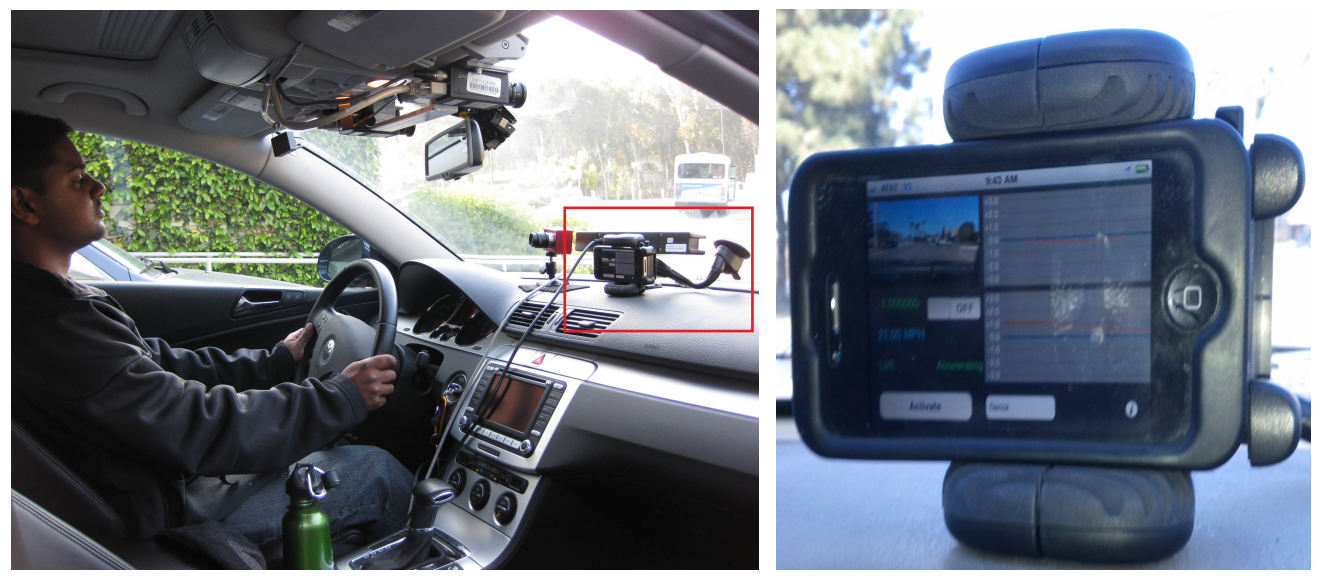
\includegraphics[width=0.7\textwidth]{images/miroad.png}
\caption{Sensores utilizados no MIROAD. \cite{johnson2011driving}}
\label{miroad}
\end{figure}

O MIROAD coleta dados continuamente do acelerômetro e giroscópio para detectar algumas manobras específicas, como curvas acentuadas
e acelerações e freadas instantâneas.
Um experimento foi feito e obteve cerca de 97\% de corretude. Estes resultados demonstram que é possível construir
um mecanismo para predição de comportamento veicular utilizando apenas sensores do smartphone e contribuem para a motivação deste trabalho.

\citeonline{eren2012estimating} apresentam um trabalho semelhante que tenta estimar o comportamento na direção de motoristas como seguro ou
não seguro, utilizando algoritmo de detecção de melhor caminho e classificação Bayesiana. Este sistema utiliza
apenas sensores de smartphone (acelerômetro, giroscópio e magnetômetro) para adquirir dados de contexto e obteve
resultados corretos em 14 casos de 15.

\citeonline{park2016integrated} desenvolveram um sistema integrado com direção veicular chamado de IDAS para conduzir estudos de experiência
do usuário (UX). Este sistema coleta dados do motorista e do veículo, analiza-os e provê um feedback visual baseado
nas informações que o motorista precisa no momento. São utilizados sensores vestíveis para aquisição de dados
fisiológicos e de movimentação do motorista, um dispositivo OBD para obtenção de dados veiculares, um GPS veicular e as informações
são exibidas em um aplicativo Android. O setup utilizado é mostrado na figura \ref{idas}.

\begin{figure}[htb]
\centering
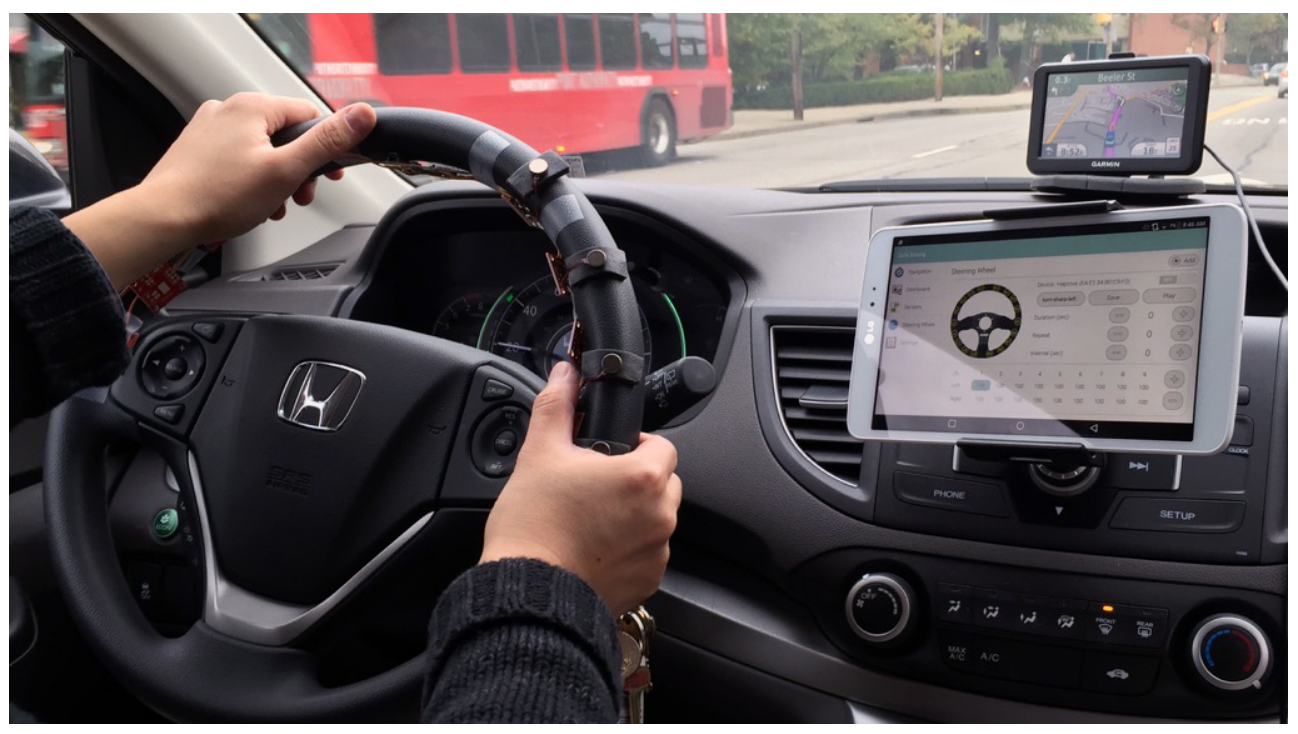
\includegraphics[width=0.7\textwidth]{images/idas.png}
\caption{Sensores utilizados no IDAS. \cite{park2016integrated}}
\label{idas}
\end{figure}

Trabalhos anteriores também corroboram a tese de que é possível utilizar sensores para prever a interruptibilidade
humana em um dado momento. \citeonline{fogarty2005predicting} construíram um modelo que utiliza sensores de áudio e vídeo
para estimar a interruptibilidade de trabalhadores de escritório em um dado momento. \citeonline{hudson2003predicting}
construíram um modelo semelhante utilizando os mesmos sensores e obtiveram uma média de 75\% de acurácia na predição de
interruptibilidade de trabalhadores de escritório.

O presente trabalho propõe um módulo que funcionará junto a um aplicativo pré-existente com o objetivo de identificar momentos
oportunos e inoportunos para interrupção de motoristas. O próximo capítulo apresenta mais detalhes sobre a arquitetura e
implementação do referido módulo.

\xchapter{Uma módulo para identificação de momentos oportunos e inoportunos para interrupção de motoristas}{}
\label{solucao}

Neste trabalho apresentamos um módulo de identificação de momentos oportunos e inoportunos para interrupção de
motoristas, usando apenas sensores de smartphone. As seções estão estruturadas da seguinte forma: A seção
\ref{sec-arquitetura-solucao} apresenta a arquitetura do módulo proposto.

\section{Arquitetura}
\label{sec-arquitetura-solucao}
Segundo \citeonline{garlan1993introduction}, a arquitetura de um software é a coleção de seus componentes computacionais - ou simplesmente
componentes - junto com a descrição das interações entre estes componentes - os conectores.  Sendo assim, nesta sessão
vamos mostrar os principais elementos da solução proposta e como eles interagem entre si.

O módulo funcionará em conjunto com o aplicativo Meu Possante, um aplicativo para sistemas Android e cuja arquitetura pode ser vista
na seção \ref{meupossante-app}. A identificação dos momentos oportunos e inoportunos é feita usando apenas sensores de smartphone,
sendo que os momentos oportunos são medidos utilizando o sensor de GPS, enquanto os inoportunos usam o giroscópio.

Os momentos escolhidos foram os seguintes:

\begin{itemize}
  \item Momentos Oportunos:
    \begin{itemize}
      \item Veículo parado \cite{kim2015sensors}
      \item Velocidade constante e menor que 29,5 km/h \cite{kim2015sensors}
    \end{itemize}
  \item Momentos Inoportunos:
    \begin{itemize}
      \item Durante uma curva \cite{monk2004recovering}
      \item Durante uma mudança de faixa \cite{monk2004recovering}
    \end{itemize}
\end{itemize}

A arquitetura solução 

%\xchapter{Proposta}{}
\label{proposta}

Neste trabalho é proposto um sistema de notificação sensível ao contexto com identificação de momentos oportunos e
inoportunos para interrupção de motoristas, usando apenas sensores de smartphone. As seções deste capítulo estão
estruturadas da seguinte forma: A seção \ref{meupossante} apresenta o Meu Possante, um aplicativo para motoristas
que serviu como motivação para este trabalho. A seção \ref{sec-momentos-oportunos-inoportunos} discorre sobre
os momentos oportunos e inoportunos escolhidos para a identificação no sistema. A seção \ref{sec-arquitetura-solucao}
apresenta a arquitetura da solução proposta. A seção \ref{sec-implementacao} mostra detalhes da implementação
de cada módulo que compõe a solução.

\section{Meu Possante}{}
\label{meupossante}
Mecânica automotiva é um assunto extremamente complexo. Cada um dos inúmeros componentes
do automóvel tem seu próprio ciclo de vida e devem ser revisados e trocados em seu próprio
tempo. Além disso, certas condições de uso podem diminuir a vida útil de algumas peças,
tornando mais frequente a necessidade de revisão.

A falta de conhecimento destes fatos pode levar ao dono de um automóvel negligenciar
as manutenções no tempo correto, causando desde transtornos que poderiam ser facilmente
evitados a acidentes ocasionados por falhas mecânicas.

Em 2016, mais de 2 milhões de automóveis foram vendidos no Brasil
\cite{fenabrave}. Dentre este número, é seguro assumir que poucos de seus
proprietários são especialistas em mecânica e possuem dúvidas sobre o
funcionamento das peças do seu veículo, além de não saber exatamente em qual
momento deve-se trocar cada uma de suas peças. Estas informações geralmente
estão no manual do veículo, mas é inviável para uma pessoa leiga memorizar
todas estas informações.

Após a compra de um automóvel, a sua manutenção é de inteira responsabilidade
do proprietário. Todas as operações de manutenção, especificadas pelo fabricante,
devem ser realizadas dentro dos intervalos apropriados \cite{manualhyundai}.
Proporcionar manutenção apropriada para o veículo, não somente reduz os custos
operacionais, mas também ajuda a impedir mau funcionamento devido a negligência,
caso que geralmente não é coberto por garantia \cite{manualonix}.

Para executar a manutenção apropriadamente, o proprietário precisa estar
sempre atento ao momento correto da troca das peças, que muda de acordo
com as condições de uso de um carro. Acompanhar estas diferentes variáveis pode
ser difícil para pessoas comuns.

O uso de um aplicativo para celular pode ser uma grande ajuda na decisão de quando
é necessário a revisão e troca de peças, alertando o usuário visualmente quando alguma
manutenção está próxima. Neste sentido surge o Meu Possante, um aplicativo que monitora
o estado atual do veículo e avisa o momento em que as manutenções das peças serão
necessárias.

O Meu Possante possui um objetivo simples: Auxiliar o motorista a identificar quais
peças de seu carro precisarão de manutenção em um futuro próximo. O aplicativo nasceu
como trabalho final da disciplina de Desenvolvimento de Aplicações para Dispositivos
Móveis e está em processo refinamento para publicação na Google Play Store.

A tela principal do aplicativo mostra todos os componentes do veículo que são monitorados,
como pode ser visto na figura \ref{meu-possante-tela-principal}. Ao clicar em um componente,
a tela do mesmo é mostrada, com informações como a frequência de troca e quilometragem
atual.

\begin{figure}[h]
\centering
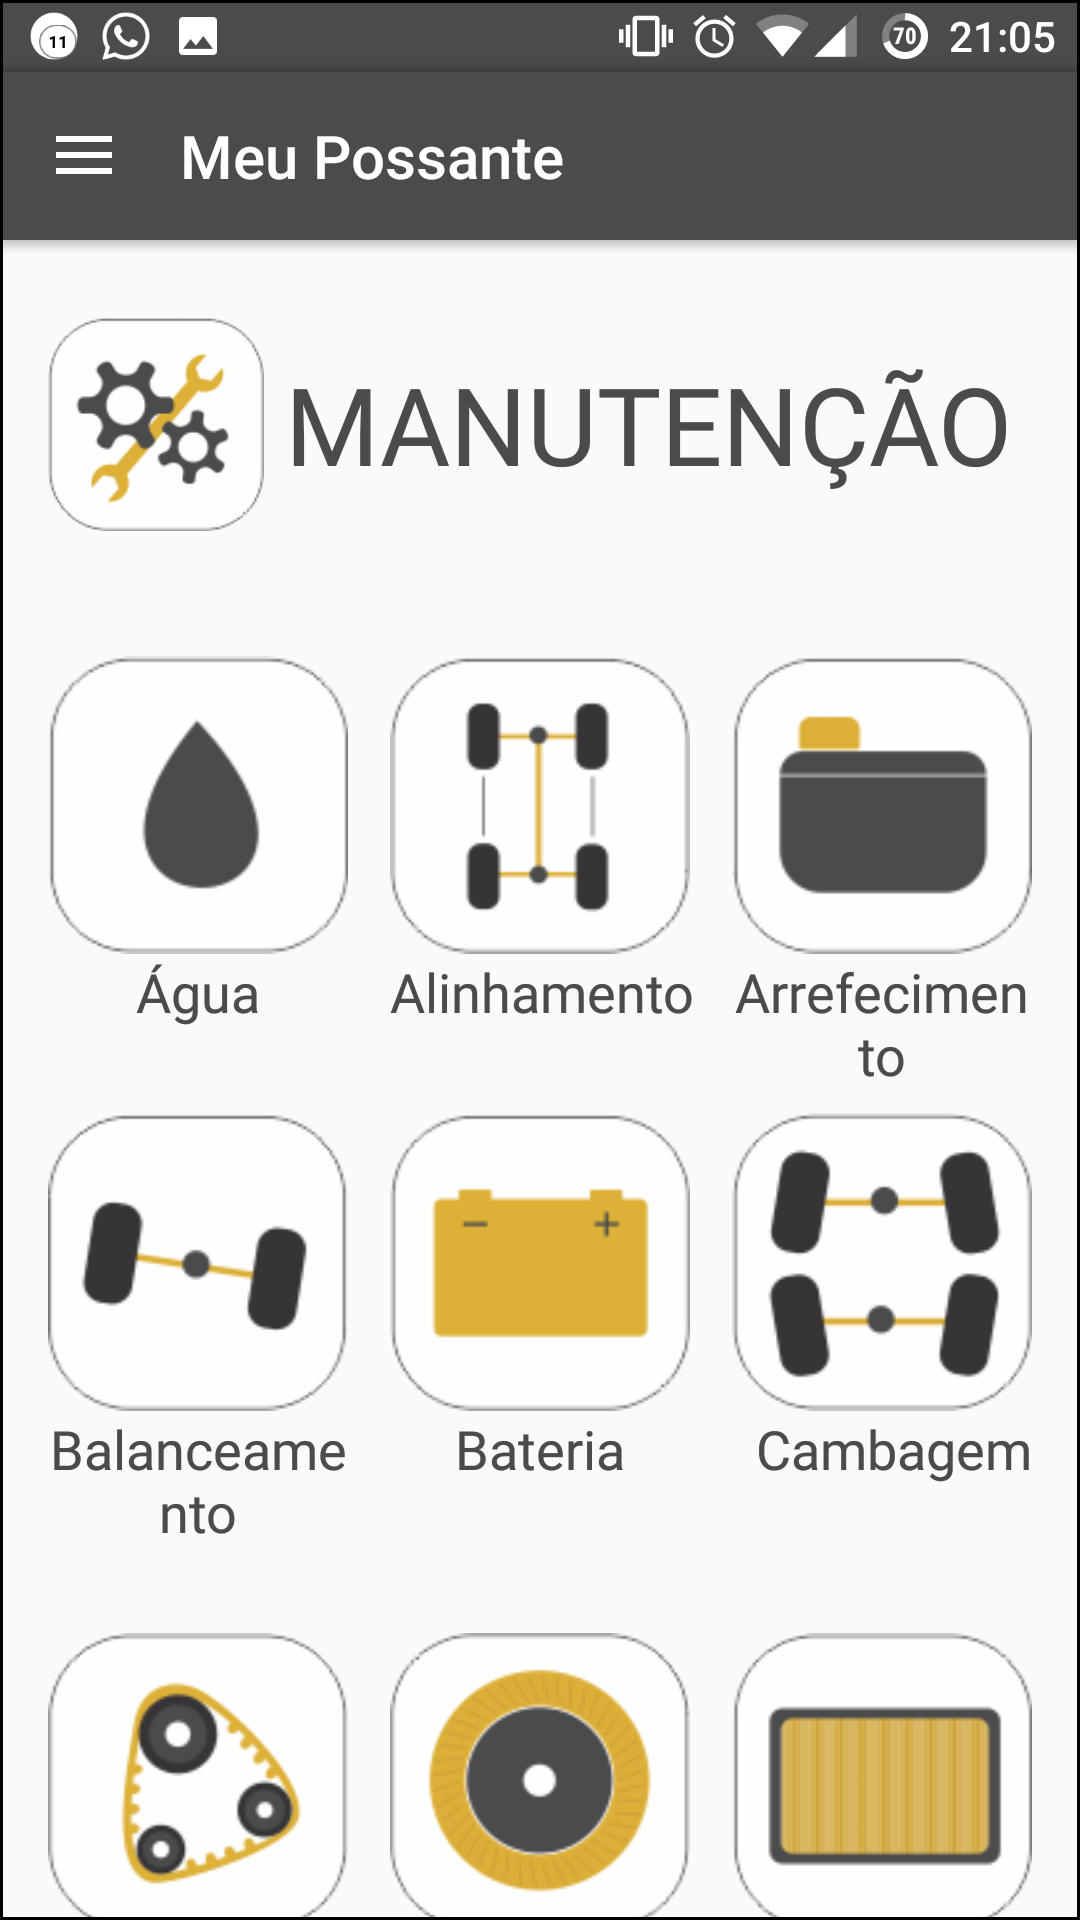
\includegraphics[width=0.3\textwidth]{images/meu-possante-tela-principal.png}
\caption{Tela principal do Meu Possante}
\label{meu-possante-tela-principal}
\end{figure}

O aplicativo utiliza informações do GPS do dispositivo para calcular a distância percorrida
pelo motorista enquanto está dirigindo. No momento em que detecta a iminência de manutenção
de alguma das peças do veículo, uma notificação é enviada para o dispositivo do usuário.
Esta notificação leva à página da peça correspondente no aplicativo, onde pode ser lido
mais detalhes sobre o estado atual, como a quilometragem e qual a quilometragem da
próxima troca, como pode ser visto na figura \ref{meu-possante-tela-componente}.

\begin{figure}[h]
\centering
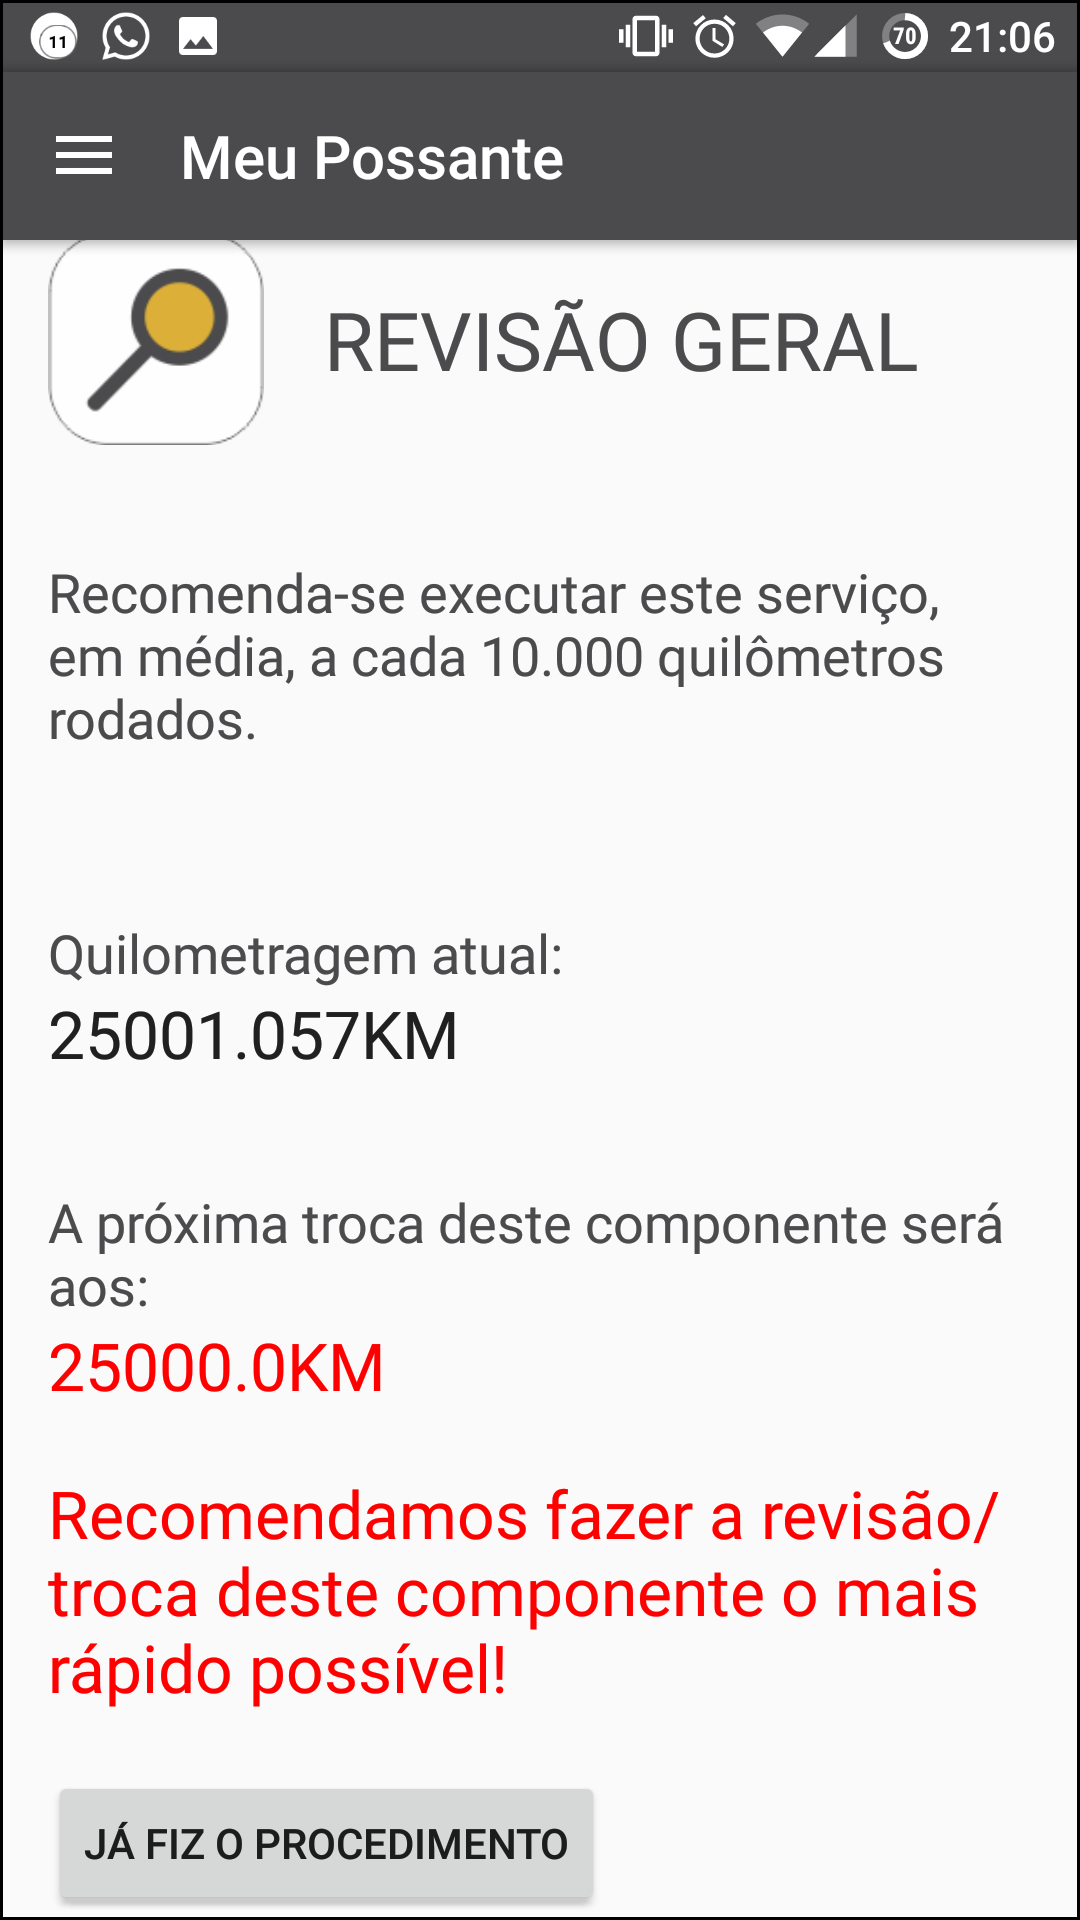
\includegraphics[width=0.3\textwidth]{images/meu-possante-tela-componente.png}
\caption{Tela que indica a necessidade de revisão de um componente}
\label{meu-possante-tela-componente}
\end{figure}

Um exemplo do caso supracitado é o fluido de freio, cuja troca recomendada é a cada
10.000 quilômetros rodados ou 1 ano, o que ocorrer primeiro. Já a troca da correia
dentada deve ser feita a cada 50.000 quilômetros, sem limite de tempo definido. Os
outros componentes funcionam da mesma forma, cada qual com sua quilometragem e
tempo de troca específicos.

Na versão atual, o motorista precisa indicar que está dirigindo através de uma tela
específica. Ao indicar que está dirigindo, o aplicativo começa a monitorar a localização
do usuário e seu deslocamento. Durante a corrida, os dados de quilometragem são atualizados
no banco de dados e na iminência da manutenção de uma peça, uma notificação é enviada para o
usuário.

\subsection{Arquitetura}
\label{meupossante-app}

O Meu Possante foi pensado de forma a ter uma arquitetura simples e eficiente. Na figura
\ref{meu-possante-arquitetura} é possível ver o fluxo de dados através dos módulos, começando pela
entrada de dados do GPS e chegando ao final com a atualização destes dados em um banco de dados
e o eventual envio de uma notificação. As setas na imagem indicam o sentido do fluxo de dados.

\begin{figure}[h]
  \centering
  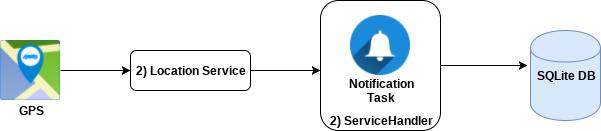
\includegraphics[width=0.7\textwidth]{images/arquitetura-meu-possante.png}
  \caption{Arquitetura do Meu Possante}
  \label{meu-possante-arquitetura}
\end{figure}

Os módulos utilizados são os seguintes:

\begin{enumerate}
  \item \textbf{Location Service:} Responsável pela configuração e gerenciamento do sensor de localização (GPS).
    O monitoramento do sensor é feito através de um serviço que continua rodando no background,
    mesmo quando o usuário não está com a aplicação aberta.
  \item \textbf{Service Handler:} Responsável pela inicialização e checagem de dados dos serviços
    que estão rodando na aplicação. Este módulo também é responsável por atualizar as informações
    de quilometragem no banco de dados e notificar o usuário, caso detecte a iminência de
    manutenção de alguma peça.
\end{enumerate}

A solução proposta no presente trabalho almeja modificar esta arquitetura para que o aplicativo não notifique motoristas
em momentos inoportunos, evitando colocá-los em potenciais riscos. A próxima seção apresenta os momentos oportunos
e inoportunos escolhidos para serem identificados.

\section{Momentos oportunos e inoportunos escolhidos}
\label{sec-momentos-oportunos-inoportunos}

Para a escolha dos momentos oportunos e inoportunos que a proposta iria identificar, foi feita uma prospecção dos artigos
existentes nessa área. Nesta etapa dois artigos se mostraram promissores: O de \citeonline{kim2015sensors} e o
de \citeonline{monk2004recovering}. Ambos trabalhos citam momentos oportunos e inoportunos para detecção da interruptibilidade
de motoristas. Os momentos escolhidos estão exibidos na tabela \ref{tabela-momentos-oportunos-inoportunos}.

\begin{table}[h]
\centering
\caption{Momentos oportunos e inoportunos escolhidos para identificação na proposta}
\label{tabela-momentos-oportunos-inoportunos}
\begin{tabular}{|c|c|}
\hline
\textbf{Momentos Oportunos}                                                & \textbf{Momentos Inoportunos} \\ \hline
Veículo parado                                                             & Curva                         \\ \hline
\begin{tabular}[c]{@{}c@{}}Veículo com velocidade\\ constante\end{tabular} & Mudança de faixa              \\ \hline
\end{tabular}
\end{table}

As próximas subseções explicam com detalhes o porquê das escolhas destes momentos.

\subsection{Momentos oportunos}
\label{subsec-momentos-oportunos}

\citeonline{kim2015sensors} desenvolveram um classificador utilizando aprendizagem de máquina para detectar a interruptibilidade
de motoristas em um dado momento. O resultado do trabalho mostrou que interrupções têm menos impacto em um motorista quando ele
não está com nenhuma das mãos no volante ou quando está interagindo com um periférico (controlador do ar condicionado, por exemplo).

Além disso, pode-se inferir a partir do trabalho de \citeonline{kim2015sensors} alguns outros momentos que são oportunos para
interromper motoristas, como por exemplo quando o carro está parado (todas as vezes em que o motorista não tinha nenhuma das
mãos no volante, a velocidade do carro era menor do que 3 km/h), quando a velocidade do veículo é baixa (durante a interação com
periféricos a velocidade do carro reduzia para cerca de 29,5 km/h) e quando a velocidade é constante.

Com base nestes achados, foi decidido que os momentos oportunos a serem detectados neste trabalho são:

\begin{itemize}
  \item Veículo parado;
  \item Veículo com velocidade menor do que 29,5 km/h e constante (sem aceleração ou desaceleração).
\end{itemize}

\subsection{Momentos inoportunos}
\label{subsec-momentos-inoportunos}

\citeonline{monk2004recovering} estudaram o efeito das interrupções e as distrações que elas causam nos motoristas.
Eles concluem em seu estudo que interrupções durante uma tarefa ou sub-tarefa trazem problemas, e cita curvas, mudanças
de faixa e entrada em uma rodovia como exemplos de sub-tarefas que o motorista executa. Logo, não é indicado notificar
um motorista durante estas atividades.

Com base nestas afirmações, os seguintes momentos inoportunos foram escolhidos para serem detectados no presente trabalho:

\begin{itemize}
  \item Curva;
  \item Mudança de faixa.
\end{itemize}

\section{Arquitetura}
\label{sec-arquitetura-solucao}
Segundo \citeonline{garlan1993introduction}, a arquitetura de um software é a coleção de seus componentes computacionais - ou simplesmente
componentes - junto com a descrição das interações entre estes componentes - os conectores.  Sendo assim, nesta sessão
vamos mostrar os principais elementos da solução proposta e como eles interagem entre si.

O módulo funcionará em conjunto com o aplicativo Meu Possante, um aplicativo para sistemas Android e cuja arquitetura pode ser vista
na seção \ref{meupossante-app}. A identificação dos momentos oportunos e inoportunos é feita usando apenas sensores de smartphone,
sendo que os momentos oportunos são medidos utilizando o sensor de GPS, enquanto os inoportunos usam o giroscópio.

O fluxo de dados da aplicação pode ser visto na figura \ref{arquitetura-meu-possante-com-modulo}. O fluxo começa
na coleta de dados do GPS e giroscópio, e termina na decisão de notificação ou não do usuário. As setas na
imagem representam o sentido do fluxo de dados.

\begin{figure}[h]
\centering
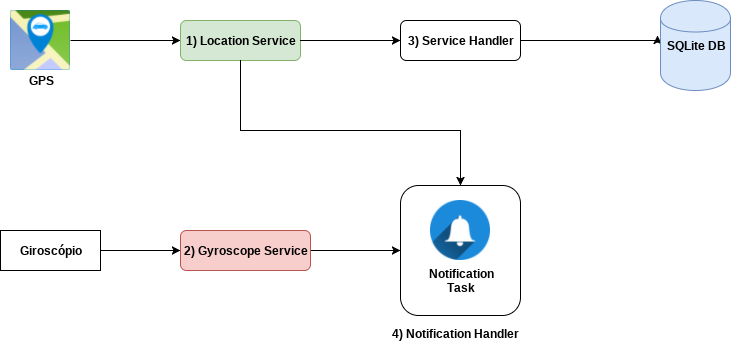
\includegraphics[width=0.85\textwidth]{images/arquitetura-meu-possante-com-modulo.png}
\caption{Arquitetura do Meu Possante após a implementação do módulo de identificação}
\label{arquitetura-meu-possante-com-modulo}
\end{figure}

Os módulos representados e suas funções são os seguintes:

\begin{enumerate}
  \item \textbf{Location Service:} Responsável pela coleta e monitoramento dos dados do GPS, incluindo deslocamento, velocidade e
  aceleração do dispositivo.
  \item \textbf{Gyroscope Service:} Responsável pela coleta e monitoramento dos dados do giroscópio. Este serviço detecta mudanças
  nos valores do sensor e aplica o algoritmo de detecção de curvas e mudanças de faixa.
  \item \textbf{Service Handler:} Responsável pela inicialização e checagem de dados dos serviços
  que estão rodando na aplicação. Este módulo também é responsável por atualizar as informações
  de quilometragem no banco de dados e chamar o módulo de notificação quando necessário.
  \item \textbf{Notification Handler:} Responsável por consultar os serviços e decidir se deve criar uma notificação ou não naquele
  momento.
\end{enumerate}

Na próxima seção são dados mais detalhes sobre os principais módulos implementados na proposta, assim como os algoritmos utilizados.

\section{Implementação}
\label{sec-implementacao}

O projeto foi desenvolvido no Android Studio, o ambiente de desenvolvimento integrado (IDE) oficial para
codificação de aplicativos Android. A linguagem utilizada foi o Java, linguagem padrão para o desenvolvimento
de aplicações Android.

As próximas subseções apresentam detalhes sobre a implementação dos principais módulos que compõem o sistema.

\subsection{Location Service}
\label{location-service}

O módulo \textit{Location Service} é o serviço responsável pela obtenção dos dados de GPS da aplicação. Os principais dados calculados
por este serviço são a distância percorrida desde a última leitura, o valor da velocidade e a aceleração. Esta última é necessária
apenas para determinar se a velocidade é constante ou não.

Por ser necessário obter a localização do usuário em intervalos regulares, foi preciso especificar o intervalo de tempo que o
serviço requisita atualizações da localização. Esta configuração tem impacto direto na autonomia de bateria do dispositivo,
pois quanto mais frequente é a requisição de dados do GPS, mais energia é gasta pelo dispositivo. O intervalo de tempo escolhido
foi de 5000ms (5 segundos), um intervalo razoavelmente frequente e que preserva a autonomia de bateria.

A distância percorrida é um dado necessário para o Meu Possante calcular a quilometragem percorrida pelo veículo até o momento e
sinalizar as trocas de peças quando necessário. Já os valores de velocidade e aceleração são necessários para determinar se um
momento é oportuno ou inoportuno para notificar um motorista. A relação entre os momentos e os dados que são usados para
identificá-los estão relacionados na tabela \ref{tabela-momentos-dados}.

\begin{table}[h]
\centering
\caption{Relação entre momentos oportunos e dados necessários para identificá-los}
\label{tabela-momentos-dados}
\begin{tabular}{|c|c|}
\hline
\textbf{Momento oportuno}                     & \textbf{Dado do serviço utilizado} \\ \hline
Veículo parado                                & Velocidade                         \\ \hline
Velocidade constante e menor do que 29,5 km/h & Velocidade e aceleração            \\ \hline
\end{tabular}
\end{table}

Mais informações sobre os referidos momentos podem ser lidas na seção \ref{sec-momentos-oportunos-inoportunos}.

Dois métodos importantes deste módulo são o \lstinline[basicstyle=\ttfamily\color{black}]|isAccelerating()|, que retorna um valor
booleano que julga se o veículo está acelerando ou não, e o método \lstinline[basicstyle=\ttfamily\color{black}]|getLastSpeed()|, que
retorna a última velocidade medida do veículo. Estes dois métodos são utilizados pelo módulo \textit{Notification Handler} para decidir se
a notificação pode ser disparada ou não.

Os valores de velocidade e distância percorrida são dados por métodos padrões da API Location, a API padrão para se trabalhar
com dados de geo-referenciamento em Android. Entretanto, não há um método padrão nesta API para medir a aceleração, e por este
motivo foi necessária a criação de um método para calculá-la. O método foi estruturado da seguinte forma:

\begin{enumerate}
  \item As últimas 5 leituras de velocidade são sempre guardadas;
  \item Verifica-se a variação de velocidade entre elas;
  \item Caso a variação entre uma leitura e sua subsequente seja menor do que 5 km/h mais o desvio padrão das leituras em questão,
  considera-se que a velocidade é constante naquele momento.
\end{enumerate}

Caso a aceleração seja constante e a velocidade seja menor que 29,5 km/h, significa que o momento é oportuno para notificar o motorista.

\subsection{Gyroscope Service}
\label{gyroscope-service}

Este serviço é o responsável pela obtenção dos dados de giroscópio. Este é o módulo mais complexo desta proposta, por ser o responsável por
detectar se o veículo está fazendo uma curva ou mudança de faixa usando apenas os dados do giroscópio. O algoritmo usado para identificar
estes dois momentos inoportunos foi desenvolvido por \citeonline{chen2015invisible} e adaptado para este trabalho.

\citeonline{chen2015invisible} relatam em seu trabalho que quando um carro muda de direção (ex: ao mudar de faixa, fazer uma curva ou passar
por rodovias sinuosas), o eixo Z do giroscópio pode ser usado para representar a velocidade angular do veículo para aquela mudança de direção.
Eles também perceberam que o padrão das leituras deste eixo se repete para determinadas atividades, como curvas e mudanças de faixa, como pode
ser visto na figura \ref{leituras-giroscopio}.

\begin{figure}[h]
\centering
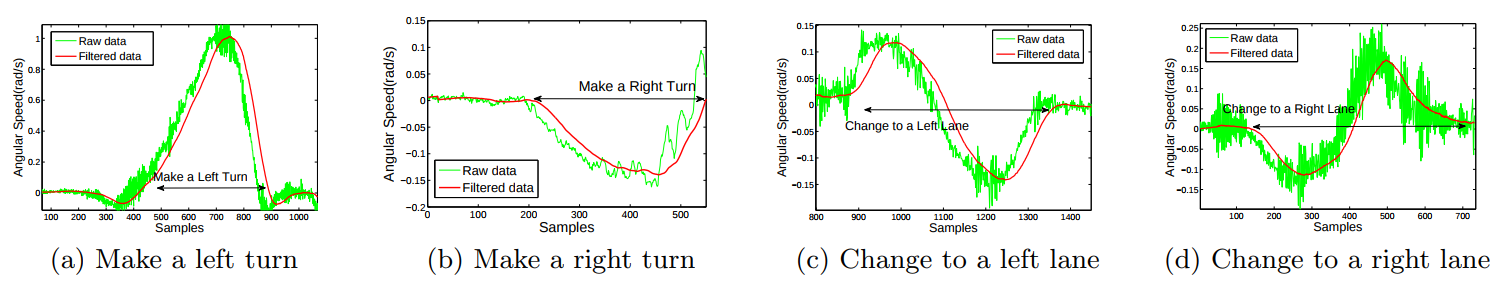
\includegraphics[width=1\textwidth]{images/leituras-giroscopio.png}
\caption{Leituras do giroscópio quando o veículo faz uma curva à direita/esquerda ou mudança de faixa à direita/esquerda \cite{chen2015invisible}}
\label{leituras-giroscopio}
\end{figure}

Pode-se observar na figura \ref{leituras-giroscopio} que as curvas são caracterizadas por uma alteração nas leituras, sendo esta positiva ou negativa,
a depender do sentido da curva; enquanto que a mudança de faixa caracteriza-se por duas alterações sequenciais, sendo a segunda no sentido inverso
da primeira.

Observando estes padrões, \citeonline{chen2015invisible} desenvolveram um conjunto de regras que determina se a alteração nas leituras do eixo Z do
giroscópio pode ser considerada um indicador de curva ou mudança de faixa. As regras são as seguintes:

\begin{enumerate}
  \item Todas as leituras durante a alteração devem ser maiores que $\delta_{s}$;
  \item O maior valor registrado durante a alteração deve ser maior do que $\delta_{h}$;
  \item A duração de uma alteração não deve ser menor do que $T_{BUMP}$.
\end{enumerate}

Através de testes e experimentos, os valores ideais encontrados por \citeonline{chen2015invisible} para as variáveis acima foram de $\delta_{s}$ = 0.05 rad/s,
$\delta_{h}$ = 0.07 rad/s e $T_{BUMP}$ = 1.5 segundos.

Considerando estas regras para o que é considerada uma alteração válida, \citeonline{chen2015invisible} desenvolveram um algoritmo baseado em mudança de estados
que tenta identificar quando o veículo está fazendo uma curva ou mudança de faixa. O algoritmo está representado na figura \ref{algoritmo-giroscopio}.

\begin{figure}[h]
  \centering
  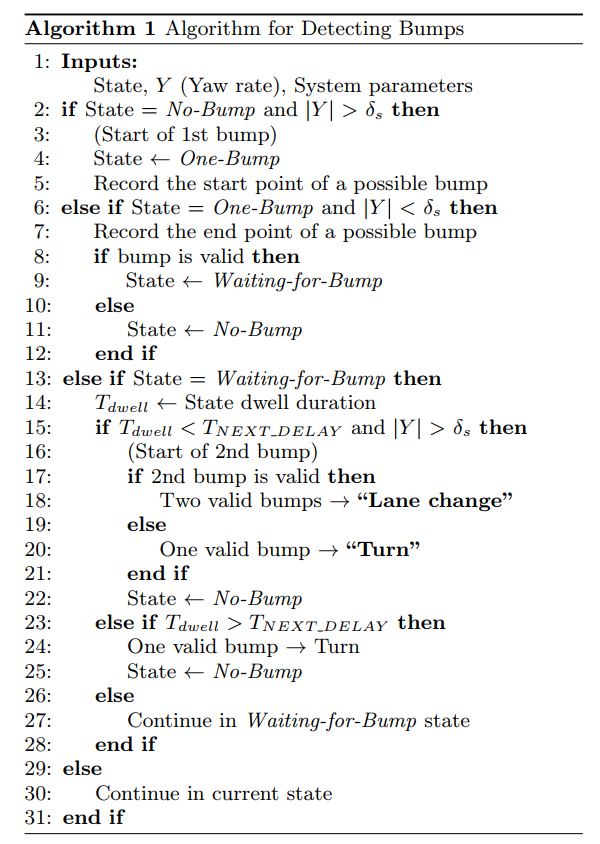
\includegraphics[width=0.45\textwidth]{images/algoritmo-giroscopio.png}
  \caption{Algoritmo de detecção de curvas e mudanças de faixa \cite{chen2015invisible}}
  \label{algoritmo-giroscopio}
\end{figure}

Os três estados do algoritmo são os seguintes:

\begin{itemize}
  \item \textbf{No-Bump:} Neste estado, nenhuma alteração foi detectada até o momento. Caso o valor do giroscópio passe de $\delta_{s}$, a alteração começa a ser
  monitorada e o estado passa a ser \textit{One Bump};
  \item \textbf{One-Bump:} Este estado começa quando o valor do giroscópio passa de $\delta_{s}$ e termina quando o valor volta a ser menor do que $\delta_{s}$.
  Caso as três regras definidas para uma alteração ser válida forem satisfeitas, o estado passa a ser \textit{Waiting-for-Bump}, caso contrário o estado volta
  a ser \textit{No-Bump}.
  \item \textbf{Waiting-for-Bump:} Este estado sucede o de \textit{One-Bump} e monitora as leituras do valor do giroscópio por um tempo de 3 segundos. Caso
  uma outra alteração comece durante esse intervalo de tempo, a alteração começa a ser monitorada. Caso ela seja válida, significa que duas alterações válidas
  ocorreram seguidamente, o que caracteriza uma mudança de faixa. Caso contrário, significa que apenas uma alteração válida ocorreu, o que caracteriza uma curva.
\end{itemize}

A solução proposta pelo presente trabalho utiliza o algoritmo de \citeonline{chen2015invisible} para detectar os momentos inoportunos de notificação: curva
e mudança de faixa. O método \lstinline[basicstyle=\ttfamily\color{black}]|isAbleToNotify()| é o responsável por informar ao módulo \textit{Notification Handler}
se o momento atual é oportuno ou não.

%% Parte pos-textual
\backmatter

% Bibliografia
% É aconselhável utilizar o BibTeX a partir de um arquivo, digamos "biblio.bib".
% Para ajuda na criação do arquivo .bib e utilização do BibTeX, recorra ao
% BibTeXpress em www.cin.ufpe.br/~paguso/bibtexpress
\bibliographystyle{abntex2-alf}
\bibliography{tcc}

% Apendices
% Comente se naoo houver apendices
% \appendix

% \xchapter{Exemplo de Ap\^endice}{} %sem preambulo
% \lipsum
% Eh aconselhavel criar cada apendice em um arquivo separado, digamos
% "apendice1.tex", "apendice.tex", ... "apendiceM.tex" e depois
% inclui--los com:
% \include{apendice1}
% \include{apendice2}
% ...
% \include{apendiceM}

%% Fim do documento
\end{document}
%------------------------------------------------------------------------------------------%
